\chapter{Convolutional Neural Networks}
\label{ch5_cnn}

Convolutional Neutral Network (CNN) is a classification of multi-layered neural networks \cite{cnn_lecun_lenet5}. CNNs have excellent performance in areas such as image recognition and classification.  CNNs are at the core of state-of-the-art approaches to a variety of computer vision tasks, including image classification \cite{kriz_suts_hinton_nips2012} and object detection \cite{gir_don_dar_mal_cvpr2014}. They are widely used in the detection and identification of faces, objects and animals, apart from powering robot vision and driverless cars \cite{cnn_karn}. LeNet-5 is one such convolutional network designed for handwritten and machine-printed character and digit recognition.

\section{Introduction}
\label{sect5_1}

\subsection{Neural Networks}
\label{sect5_1_1}
An Artificial Neural Network, simply put as Neural Network, is a computational model motivated by the manner in which neural networks in the human brain and nervous system process information \cite{cnn_karn}. The field of Neural Networks was primarily inspired by the objective of modeling biological neural systems, but has since diverged and become a part of engineering and achieving great results in machine learning \cite{nn_stanford_1}. \newline\newline The fundamental building block of a neural network is the neuron, also referred to as node. The following figures shows a biological neuron and its computational model are related: \newline

\begin{figure}[h!]
\centering
\includegraphics[width=8cm]{figures/Neuron.png}
\caption{Representation of a biological neuron\cite{nn_stanford_1}}
\label{fig:cnn1}
\end{figure}

\begin{figure}[h!]
\centering
\includegraphics[width=7cm]{figures/Neuron_Model.jpg}
\caption{Computational model of a neuron \cite{nn_stanford_1}}
\label{fig:cnn2}
\end{figure}

In this model, a node gets inputs from other node or an external source, and calculates an output. Inputs have associated weights assigned on basis of their relevance to other input nodes. The node applies a function on the weighted sum of inputs, as shown in Figure \ref{fig:cnn3}.
\begin{figure}[h!]
\centering
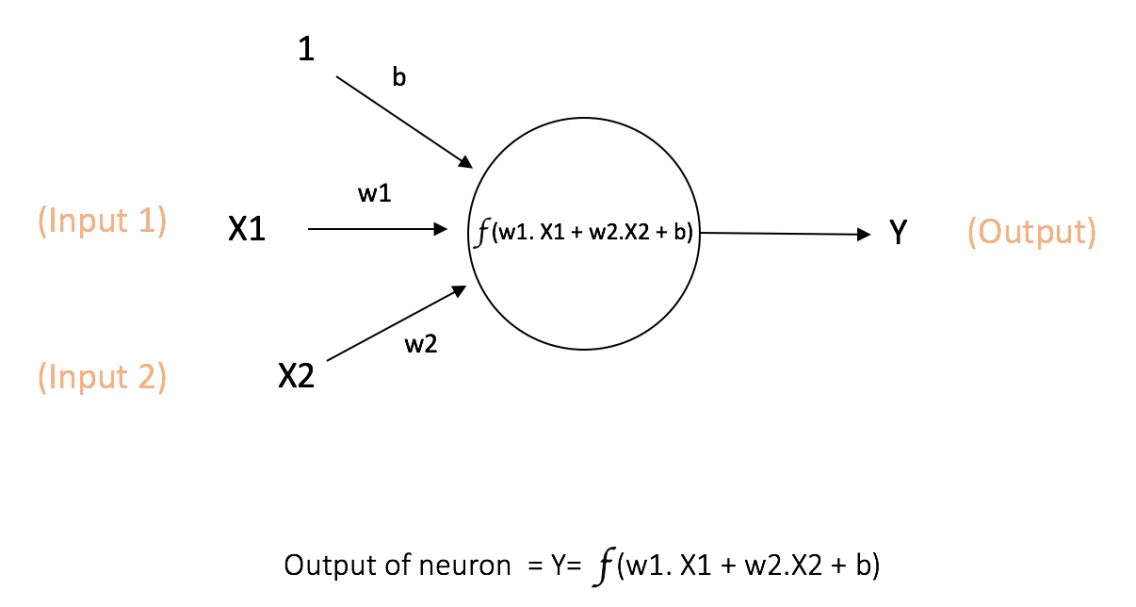
\includegraphics[width=10cm]{figures/Input_and_Output_to_a_Node.png}
\caption{Computation in a Neuron\cite{nn_karn}}
\label{fig:cnn3}
\end{figure}

The neuron receives inputs x1 and x2 with weights w1 and w2. Each neuron also has another input 1, with a weight \textbf{bias} associated with it. The bias value provides each node a trainable constant value.\newline\newline 
The function applied to the sum of weighted inputs, known as Activation Function, is a non-linear function introduced to force neurons to learn non-linear representations, as most of real world data is non-linear. Following are some common activation functions used:

\begin{itemize}
\item Sigmoid \newline
Takes a real-valued input and squeezes it in the range 0 to 1
\begin{equation}
\mathbf{\sigma(x) = 1 / (1 + exp(-x))}
\end{equation}

\item tanh \newline
Takes a real-valued input and squeezes it in the range -1 to 1
\begin{equation}
\mathbf{tanh(x) = 2 \sigma (2x)-1}
\end{equation}

\item ReLU \newline
Takes a real-valued input and thresholds it at zero (replaces negative values with zero)
f(x) = max(0, x)
\begin{equation}
\mathbf{f(x) = max(0, x)}
\end{equation}
\end{itemize}

\subsubsection{Feedforward Neural Network}
\label{sect5_1_1_1}
One of the first and simplest neural networks devised was the feedforward neural network. There are multiple neurons placed in layers, with edges connecting them. Each of these edges are tagged a weight. Figure \ref{fig:cnn4} shows an example of a feedforward neural network.\newline\newline
\begin{figure}[h!]
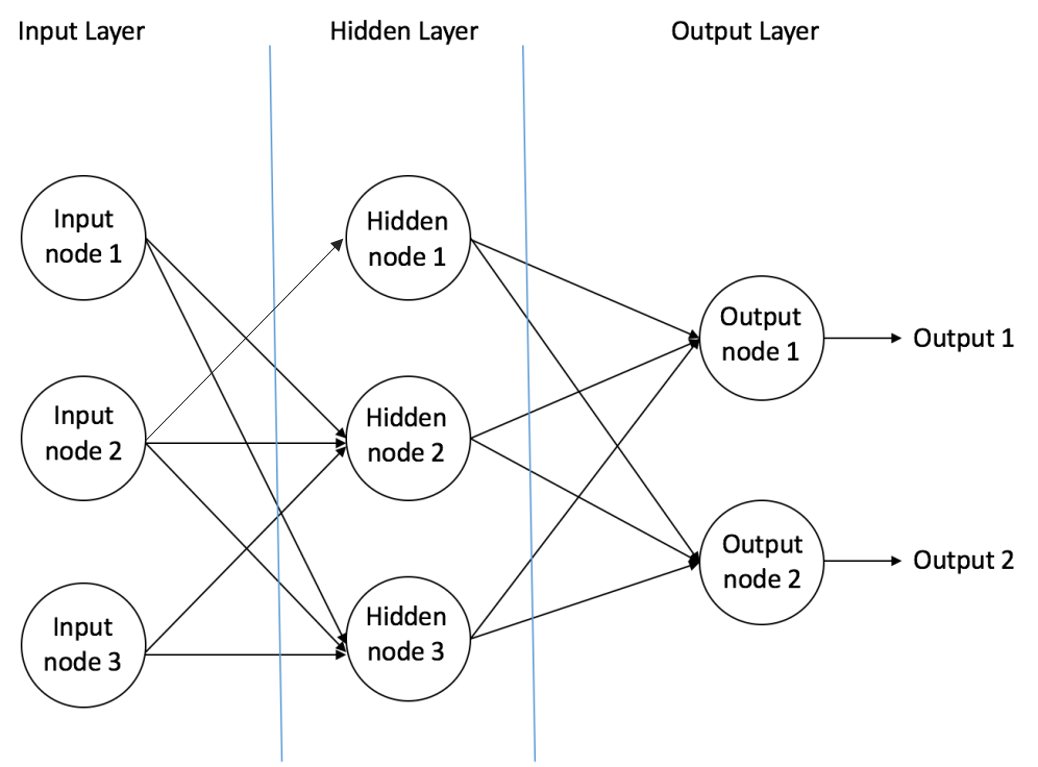
\includegraphics[width=14cm]{figures/Feedforward_Neural_Network.png}
\caption{Feedforward Neural Network \cite{nn_karn}}
\label{fig:cnn4}
\end{figure}
Information only moves in the forward direction in a feedforward neural network. Input nodes receive signals from the outside world and pass on the information forward to the hidden nodes, which perform computations and propagate information to the output nodes. The output nodes carry out some calculations and transfer the result to the outside world. There can only be one input and output layer of nodes, but multiple hidden layers of nodes in a feedforward neural network.\newline\newline 
They are of two types, \textbf{Single Layer Perceptron} and \textbf{Multi Layer Perceptron} (MLP). The former does not consist of any hidden nodes in the middle, while the the latter has at least one hidden layer. MLPs are very useful in several practical learning applications.
\subsubsection{Training}
\label{sect5_1_1_2}
For any neural network to accurately learn relationships between inputs and outputs and generate correct predictions, training is required. For an MLP to learn, back propagation algorithm is used.\newline\newline
Back-propagation is one of the many ways to train a MLP. It is a supervised learning algorithm which learns from labeled training datasets. Back-propagation algorithm trains the MLP by correcting its output when a mistake is made. Its objective is to assign correct weights to the connections between nodes in different layers, so as to generate accurate outputs. \newline\newline
In the beginning, all edge weights are assigned random values. For every input in the training dataset, the MLP is activated and its output is noticed and checked against the desired output from the labeled data. The error is then “propagated” back to the previous layer. This error is computed and the weights are updated. This process repeats until the output error is less than a pre-specified threshold.\newline\newline
Once the algorithm finishes, a “learned” neural network is created which can work with new inputs. It will have learned from millions of example inputs (labeled data) and from mistakes made in predicting outputs (error propagation).


\subsubsection{Visualisation}
\label{sect5_1_1_3}
Andy Harley developed a two-dimensional and three-dimensional representation of an MLP trained to recognise the handwritten digits from the \ac{MNIST} database \cite{harley2015isvc}. The following figure shows how a MLP is visualised in 3D.

\begin{figure}[h!]
\centering
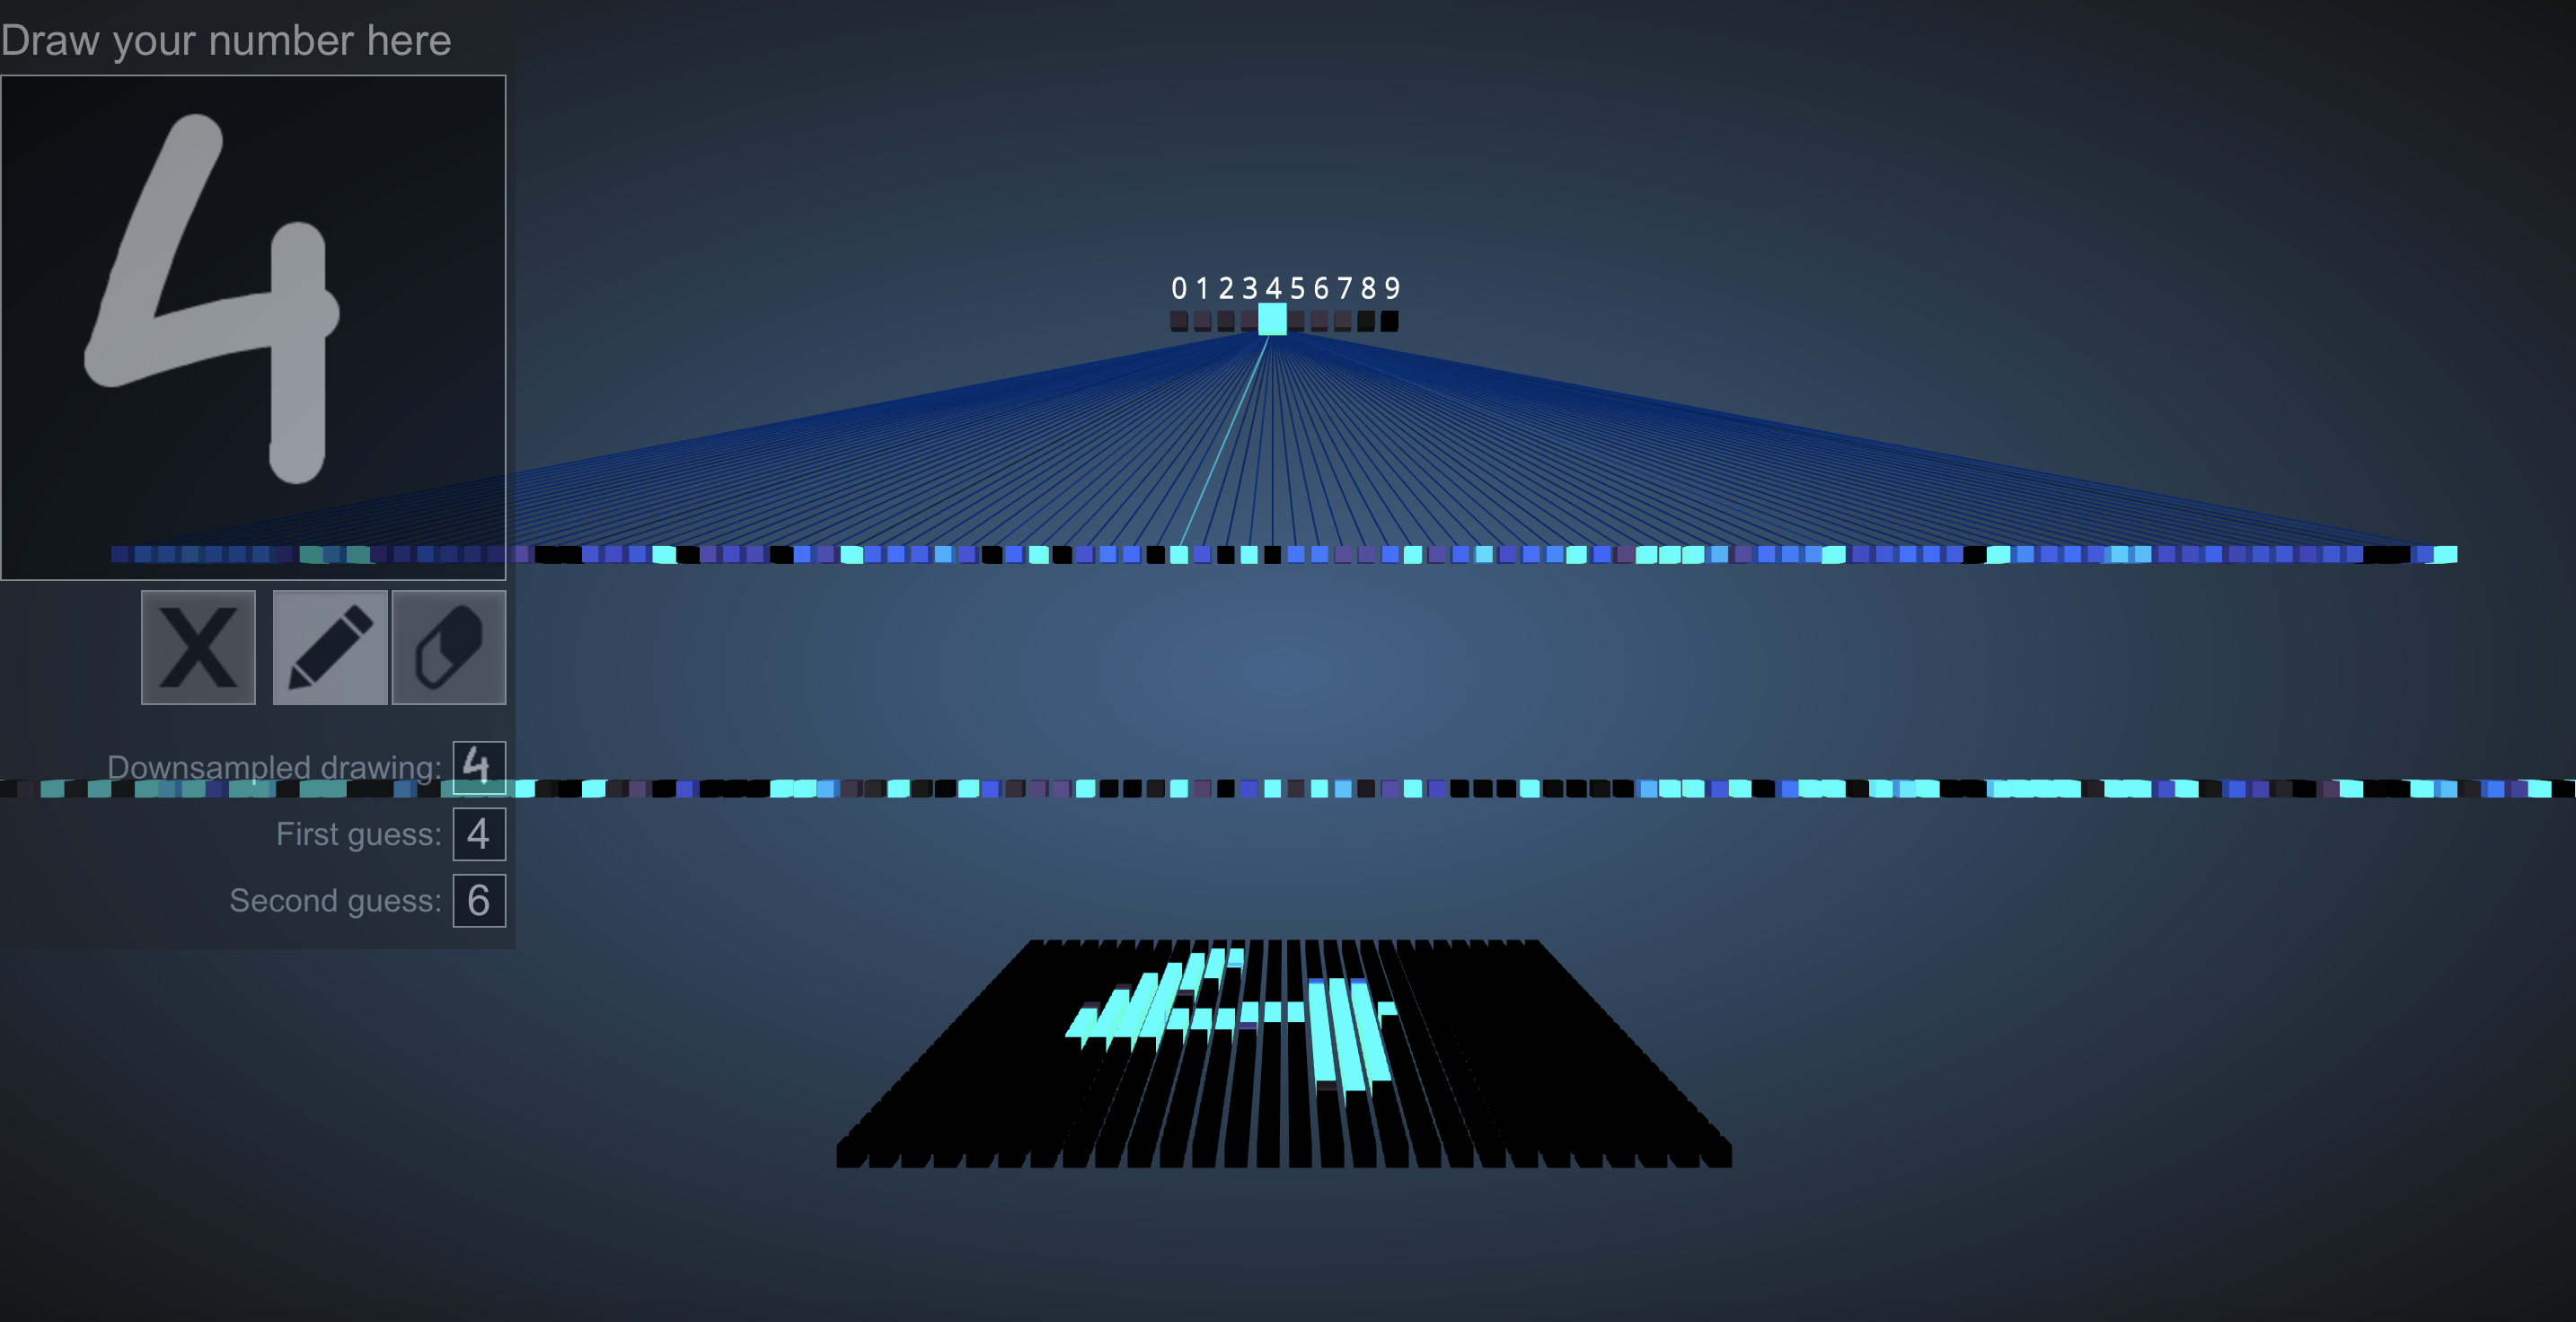
\includegraphics[width=12cm]{figures/Fully_Connected_MLP_3D.png}
\caption{3D Visualisation of a fully connected MLP \cite{harley2015isvc}}
\label{fig:cnn5}
\end{figure}

This MLP network has 784 nodes on the bottom layer (corresponding to pixels), 300 nodes in the first hidden layer, 100 nodes in the second hidden layer, and 10 nodes in the output layer (corresponding to the 10 digits)\cite{harley2015isvc}. \newline\newline
A brighter colour corresponds to a node which has a higher output value than others. In the input layer, the bright nodes are the ones receiving higher numerical pixel values as input. In the output layer, the only bright node corresponds to the digit 4, indicating that the MLP has correctly classified the input digit as 4.

\subsection{Convolutional Neural Networks}
\label{sect5_1_2}
CNNs are quite similar to regular neural networks – they are composed of neurons possessing learnable weights and biases; neurons get inputs, perform dot products and follow it up with non-linearity (optionally). The network expresses a single differentiable score function: from the raw image pixels on one end to class scores at the other. There is a loss function on the last, fully-connected layer which generates the final output. The difference exists for the type of input CNN architectures explicitly assume, which are images, allowing certain properties to be encoded into the architecture. These then make the forward function more efficient to implement and hugely decrease the number of parameters in the network \cite{cnn_stanford}.

\subsubsection{Architecture}
\label{sect5_1_2_1}
CNNs are biologically-inspired variants of MLPs. They take benefit of the fact that inputs accepted are images, and constrain the architecture in a more sensible way. Unlike a regular Neural Network, the layers of a CNN consist of neurons arranged in 3 dimensions: width, height, depth. Neurons in a layer are only be connected to a small region of the layer before it, instead of all neurons in a fully-connected way.Every layer transforms a 3D input to 3D output using some differentiable function. Eventually, the final output layer is one-dimensional, as the full image gets reduced into a single vector of class scores by the end of all processing.

\begin{figure}[h!]
\centering
\includegraphics[width=6cm]{figures/Neural_Net.png}
\hspace{7mm}
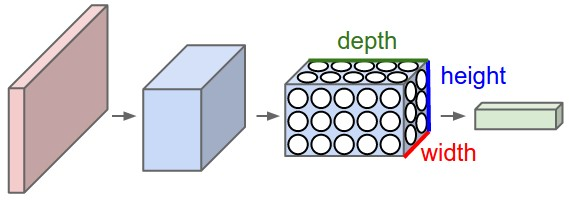
\includegraphics[width=6cm]{figures/cnn.png}
\caption{Visualisation of a Feedforward neural network \textit{(left)} and a CNN \textit{(right)}}
\label{fig:cnn6}
\end{figure}

For accuracy in predictions made by neural networks, a lot depends on how the layers are defined by the architecture. In our case, we are going to study the LeNet-5 architecture. 

\subsection*{LeNet-5 Architecture}
\label{sect5_1_2_1a}

This was one of the very first convolutional neural network, conceptualised in 1994, which propelled the field of Deep Learning. Yann LeCun, a French scientist was the person behind this pioneering work, achieved as a result of several successful iterations since 1988 \cite{cnn_culurciello}. Several new architectures have been proposed in the recent years which have improved features over LeNet, but they are all based upon the foundation of Lenet. \newline\newline
The network receives an image as an input and assigns probabilities to various output possibilities. The one with the highest probability is the classified character or digit. Following are the various steps involved in the classification process:
\begin{figure}[h!]
\centering
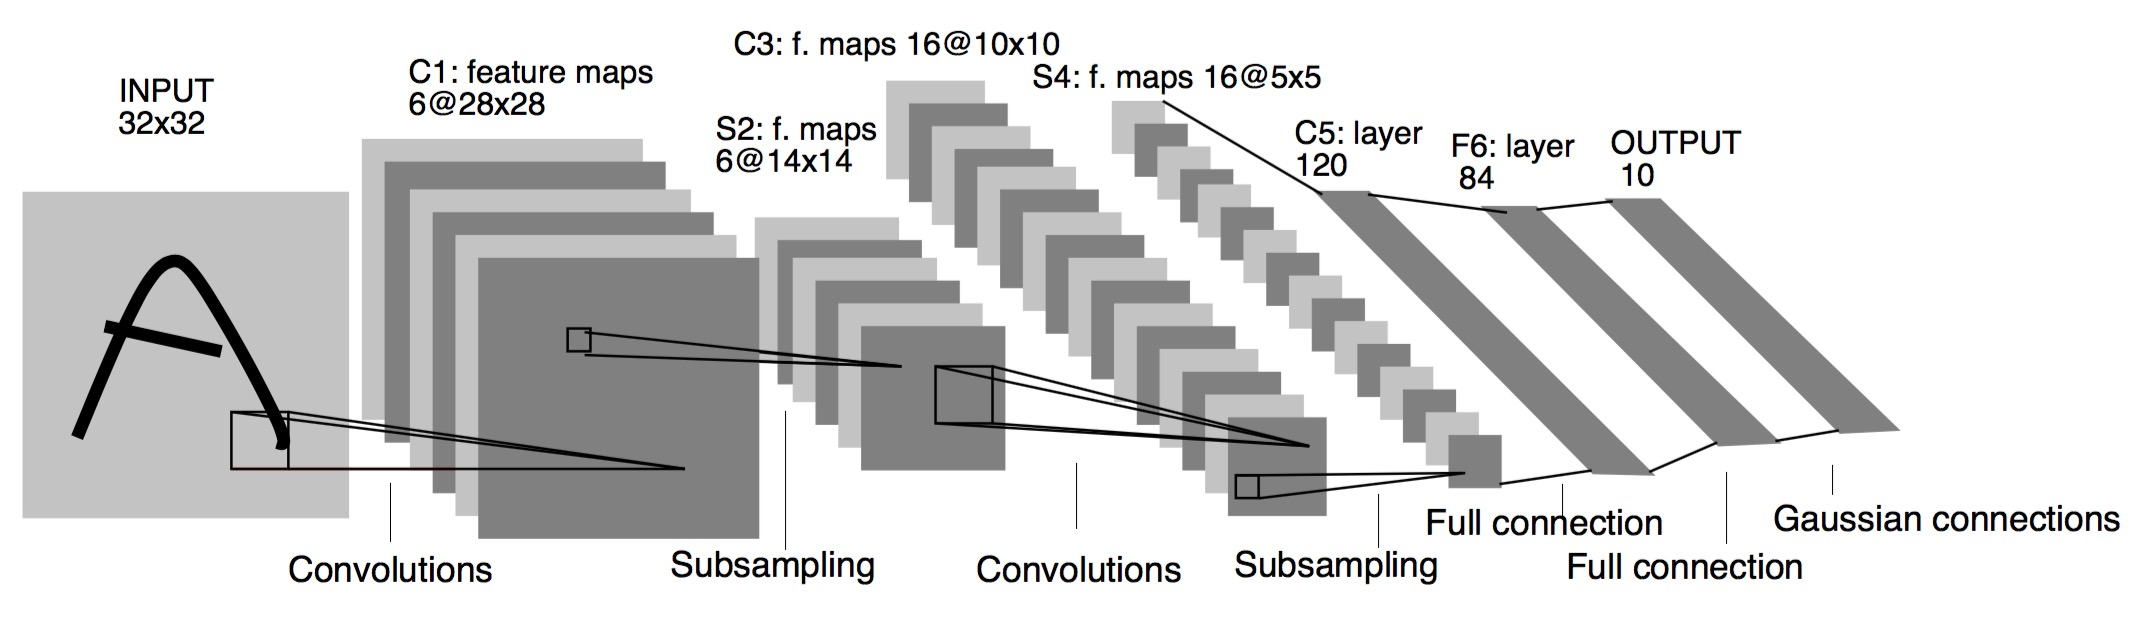
\includegraphics[width=\linewidth]{figures/Lenet5.png}
\caption{Lenet-5 architecture}
\label{fig:cnn7}
\end{figure}

The operations forming the building blocks of every convolutional neural network are as follows:
\begin{itemize}
\item Convolution
\item Pooling or Down-Sampling
\item Activation Function for Non Linearity (ReLu)
\item Classification (Fully Connected Layer)
\end{itemize}

\subsubsection*{Convolution Layer}
\label{sect5_1_2_1a_a}
Channel is a traditional term used to refer to a the coloured component of an image. A coloured image from a has three channels – red, green and blue, and could be imagined as three 2D-matrices stacked over each other (one for each color), each having pixel values in the range 0 to 255.\newline\newline
On the other hand, grayscale images have just one channel. The value of each pixel in the matrix will range from 0 to 255 – zero indicating black and 255 indicating white. Convolution layer extracts key features from the input image using convolution operations. It preserves the spatial relationship between pixels by learning image features using small squares of input data.\newline\newline
The image is convolved with multiple filters, resulting in the formation of different feature maps. Essentially, each filer is a 2D matrix (for a grayscale image), based on the value of whose individual elements, feature maps vary. \newline\newline
The orange matrix is slided over the image matrix, 1 pixel  at a time (also called ‘stride’), and for each position, an element wise multiplication is computed (between the two matrices). The multiplication outputs are added to get the final integer which makes one element of the output matrix at the corresponding position. The 3×3 filter only observes one part of the input image in each stride.\newline\newline
For example, if there is a 5x5 image convolved with a 3x3 filter as follows, a feature map will be generated based on the convolution result. For a different filter matrix, another feature map would have been generated.\newline\newline
\begin{figure}[h!]
\centering
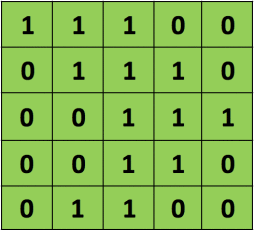
\includegraphics[width=3cm]{figures/Image.png}
\hspace{4mm}
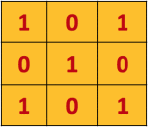
\includegraphics[width=3cm]{figures/Filter.png}
\caption{Convolution operation in action - a 5x5 Image  and a 3x3 filter}
\label{fig:cnn8}
\end{figure}

\begin{figure}[h!]
\centering
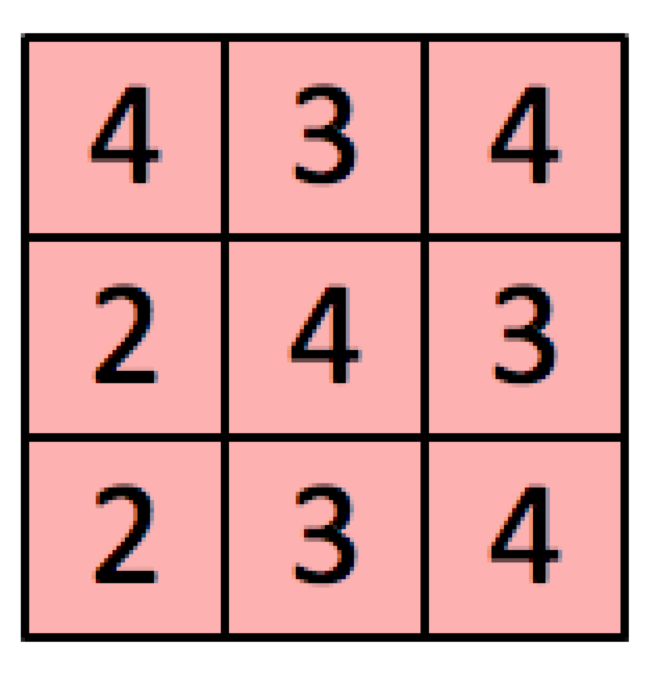
\includegraphics[width=3cm]{figures/Convolution_Result.png}
\caption{Convolution operation in action - a 5x5 Image  and a 3x3 filter}
\label{fig:cnn9}
\end{figure}

In the practical world, a CNN learns the values or weights of these filters itself during the training process. The greater the number of filters, the more image features are extracted and the better the network becomes at recognizing patterns in images, not seen previously.


\subsubsection*{Pooling Layer}
\label{sect5_1_2_1a_b}
Pooling or down-sampling reduces the dimensions of each feature map but retains the most important details. It could be done using different mathematical operations: addition, average or maximum.\newline\newline
In case of Max Pooling, a spatial neighborhood is defined (for example, a 2×2 window) and the largest element is taken from the rectified feature map within that window.
\begin{figure}[h!]
\centering
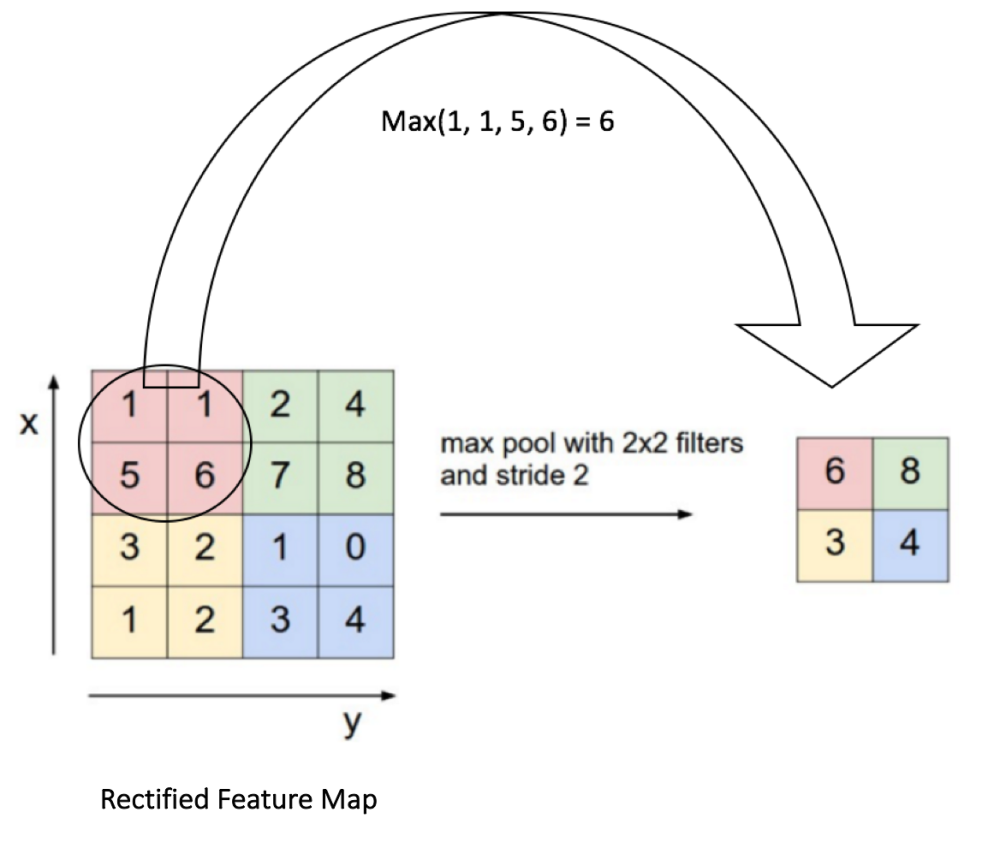
\includegraphics[width=8cm]{figures/Max_Pooling.png}
\caption{Demonstration of Max Pooling}
\label{fig:cnn10}
\end{figure}
The dimensionality of the 2-dimensional window (2x2) is also called as stride. The window is slided by the stride value, and the maximum value from that region is taken in the reduced feature map. This is how the dimensionality of the feature map decreases. Figure \ref{fig:cnn9} demonstrates how pooling reduces the size of the feature map for a sample image.
\begin{figure}[h!]
\centering
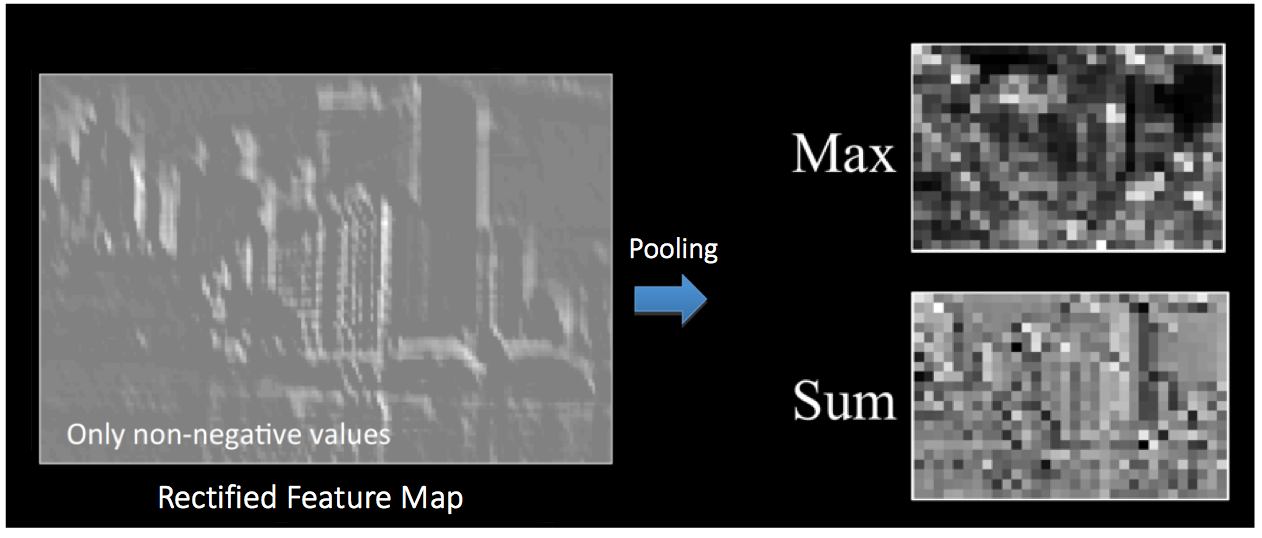
\includegraphics[width=10cm]{figures/Effect_Pooling.png}
\caption{Effect of Max Pooling layer on a sample image}
\label{fig:cnn11}
\end{figure}

\subsubsection*{Non-Linearity Layer (ReLU)}
\label{sect5_1_2_1a_c}
This is an additional layer utilised to introduce non-linearity in the image feature maps. ReLU stands for Rectified Linear Unit, which is a non-linear function.
\begin{equation}
\mathbf{Output = max(0, input)}
\end{equation}
\begin{figure}[h!]
\centering
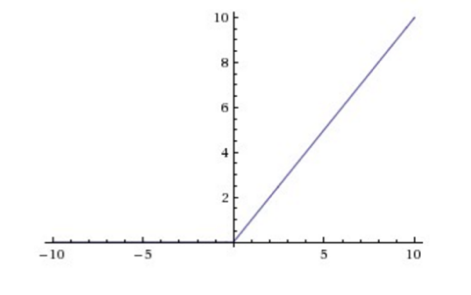
\includegraphics[width=8cm]{figures/ReLu_Layer.png}
\caption{Non-linearity operation in ReLU layer}
\label{fig:cnn12}
\end{figure}\newline
This operation is done on every single element of the image or its feature map(s), replacing every negative value with a zero.
\begin{figure}[h!]
\centering
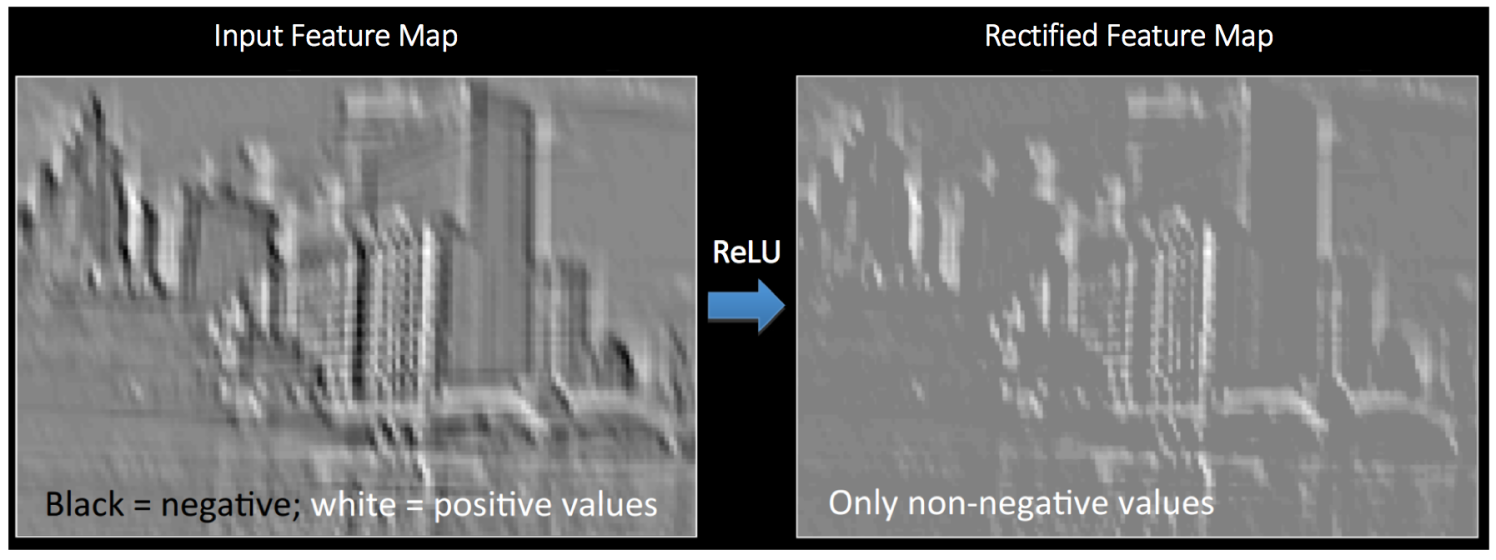
\includegraphics[width=12cm]{figures/Effect_ReLu.png}
\caption{Effect of ReLU layer on a sample image}
\label{fig:cnn13}
\end{figure}
The purpose of ReLU is to introduce non-linearity in our CNN, since most of the real-world data the network would be classifying would be non-linear. Other non-linear functions such as \textbf{tanh} or \textbf{sigmoid} could also be used as an alternative. Figure \ref{fig:cnn11} shows the effect of applying non-linearity on an image.

\subsubsection*{Fully Connected Layer}
\label{sect5_1_2_1a_d}

The fully connected layer is a classic \ac{MLP} using a softmax activation function in the output layer. Each node from the previous layer is connected to each node in the the next layer, hence the term "fully connected".\newline\newline
The output from the convolutional and pooling layers represent high-level features of the input image. The purpose of this fully connected layer is to use these features for classifying the input image into various categories, depending on the training data. \newline\newline
The sum of output probabilities from the Fully Connected Layer is 1. This is ensured by using the \textbf{softmax} as the activation function in the output layer of the Fully Connected Layer. The \textbf{softmax} function takes a vector of arbitrary real-valued scores and squashes it to a vector of values between zero and one that sum to one.

\subsection*{Training}
\label{sect5_1_2_1b}
The training of a CNN follows the same methods as those for a regular neural network. All filters and weights are assigned with random values. The network then accepts an image as its input and performs the convolution, pooling, and non-linearity operations, calculating its output probability in the end. This prediction may or may not be accurate, since the weights were assigned randomly.\newline\newline
The total error is computed at the output layer. Afterwards, back propagation is used to calculate the gradients of the error with respect to all weights in the network and gradient descent is used to update the values of all weights to minimise the output error. The weights are updated in proportion to their contribution to the total error. \newline\newline
These steps are repeated across all images present in the dataset to train the CNN completely, which results in a "learned" network. 
\subsubsection{Visualisation}
\label{sect5_1_2_2}
Along with visualising \ac{MLP}, Andy Harley developed a visualisation tool for a CNN trained to recognise handwritten digits from the MNIST database \cite{harley2015isvc} as well. \newline\newline
The following figure shows how a network can be visualised in 2D.

\begin{figure}[h!]
\centering
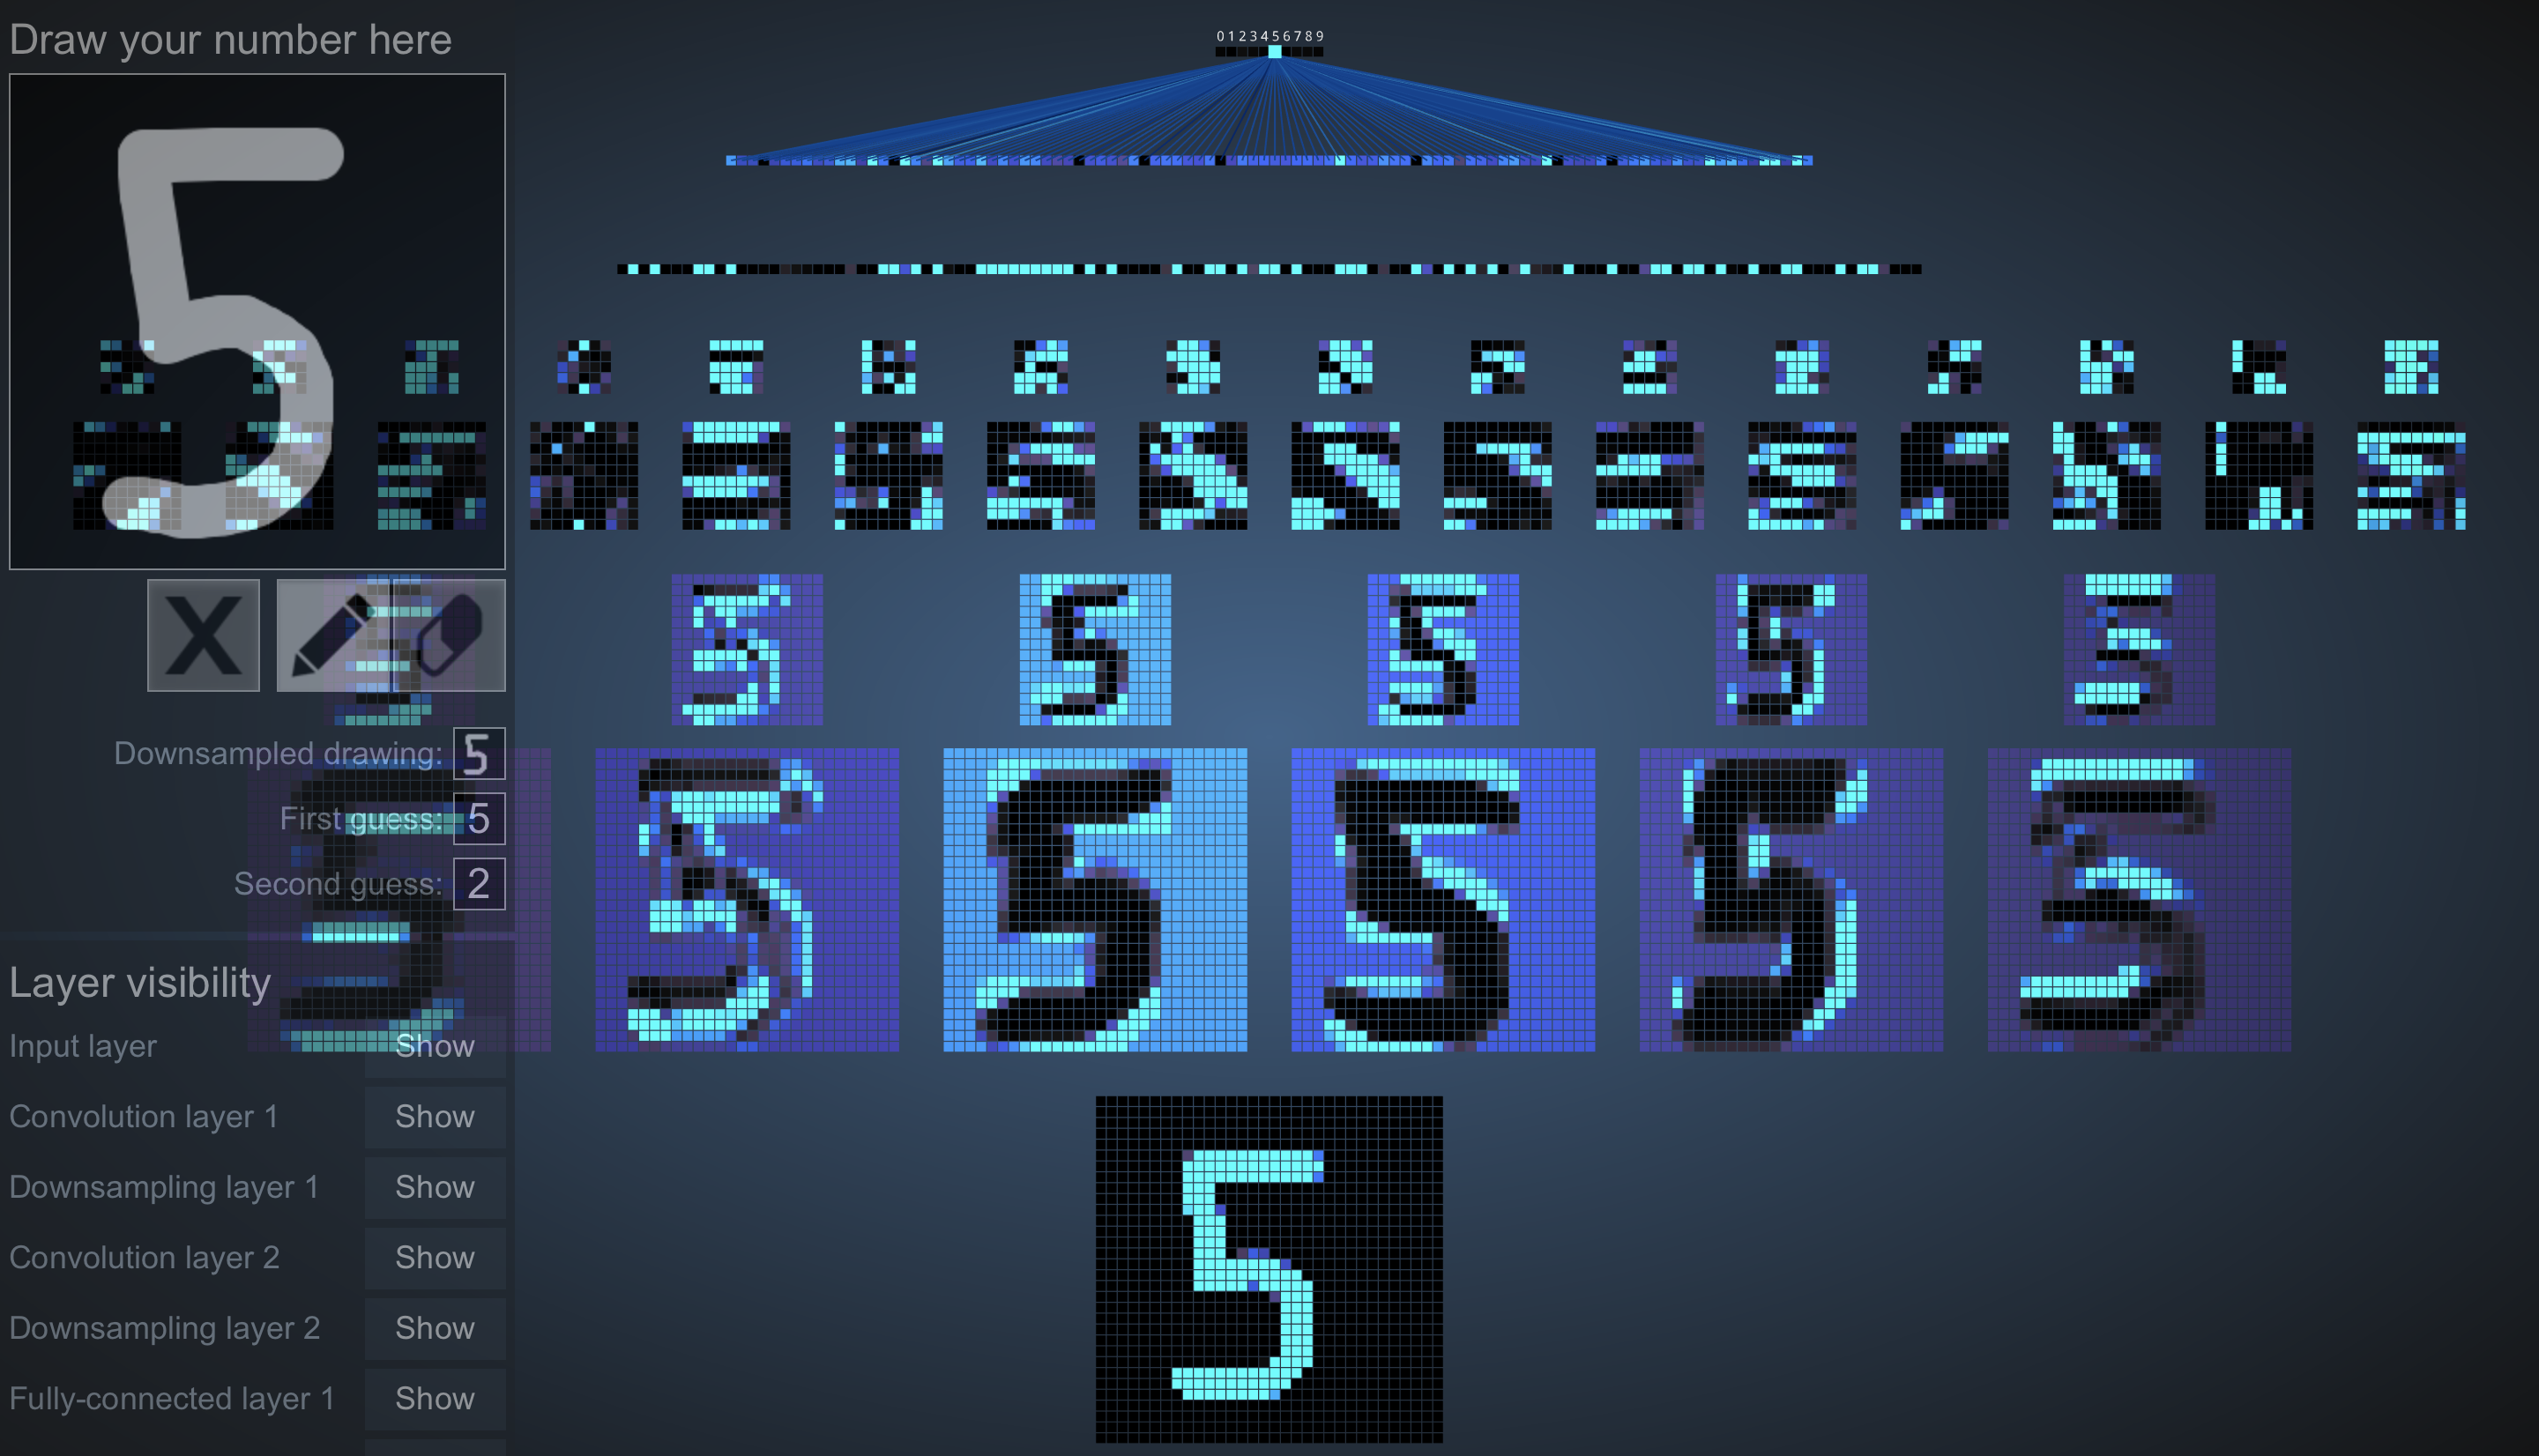
\includegraphics[width=13cm]{figures/ConvNet_2D.png}
\caption{2D Visualisation of a CNN recognising MNIST handwritten digits \cite{harley2015isvc}}
\label{fig:cnn14}
\end{figure}

This CNN has 1024 nodes on the bottom layer (corresponding to pixels), six 5x5 (stride 1) convolutional filters in the first hidden layer, followed by sixteen 5x5 (stride 1) convolutional filters in the second hidden layer, then three fully-connected layers, with 120 nodes in the first, 100 nodes in the second, and 10 nodes in the third. The convolutional layers are each followed by a downsampling layer that does 2x2 max pooling (with stride 2)\cite{harley2015isvc}.

\section{MNIST Database}
\label{sect5_2}
The \ac{MNIST} database is an enormous database of handwritten digits which is frequently utilized for training different image processing procedures \cite{mnist_wiki}. It is also extensively used for training and testing in the field of machine learning. \newline\newline 
The MNIST database consists of 60,000 training and testing images \cite{mnist_kus_ernst}. Samples from National Institute of Standards and Technology’s (NIST) original training and testing dataset were remixed to generate the MNIST database. The digits have been size-normalized and centered in a fixed-size image of 20x20 while preserving their aspect ratio \cite{cnn_lecun_mnist_app}. The resulting images contain grey levels because of anti-aliasing methods used by the normalization algorithm. The images were centred in a 28x28 image by calculating the centre of mass of the pixels and rendering the image to place this point at the centre of the 28x28 field. \newline\newline
The database is a good starting point for individuals who desire to learn machine learning techniques and pattern recognition methods on real-world data while spending marginal efforts on preprocessing and formatting. When one learns how to program, there's a tradition to print "Hello World" in his first program. Similar to how programming has Hello World, machine learning has MNIST. \newline\newline
A number of scientific papers have been written to attempt achieving the lowest error rate in predicting the digits – one paper achieves a rate as low as 0.23 percent using a hierarchical system of convolutional neural networks.

\section{Experiments}
\label{sect5_3}
An existing real word application was obtained and executed to further gauge the performance capabilities of OpenCL. An MNIST handwritten digits prediction application written by Gopala Krishna Hegde based on LeNet-5 convolutional neural networks was cloned from GitHub for this purpose \cite{cnn_mnist_papaa}. The implementation has been done in C++ as well as OpenCL.

\subsection{Analysis of Application Code}
\label{sect5_3_1}
After understanding how the LeNet-5 architecture works, the application was studied and the sizes and computations of the various layers within the CNN were determined. For each layer, mathematical operations like add, substract, multiply, divide and finding the maximum of two numbers were counted as operations.\newline\newline
The layers in the network can be represented as follows:
\begin{figure}[h!]
\centering
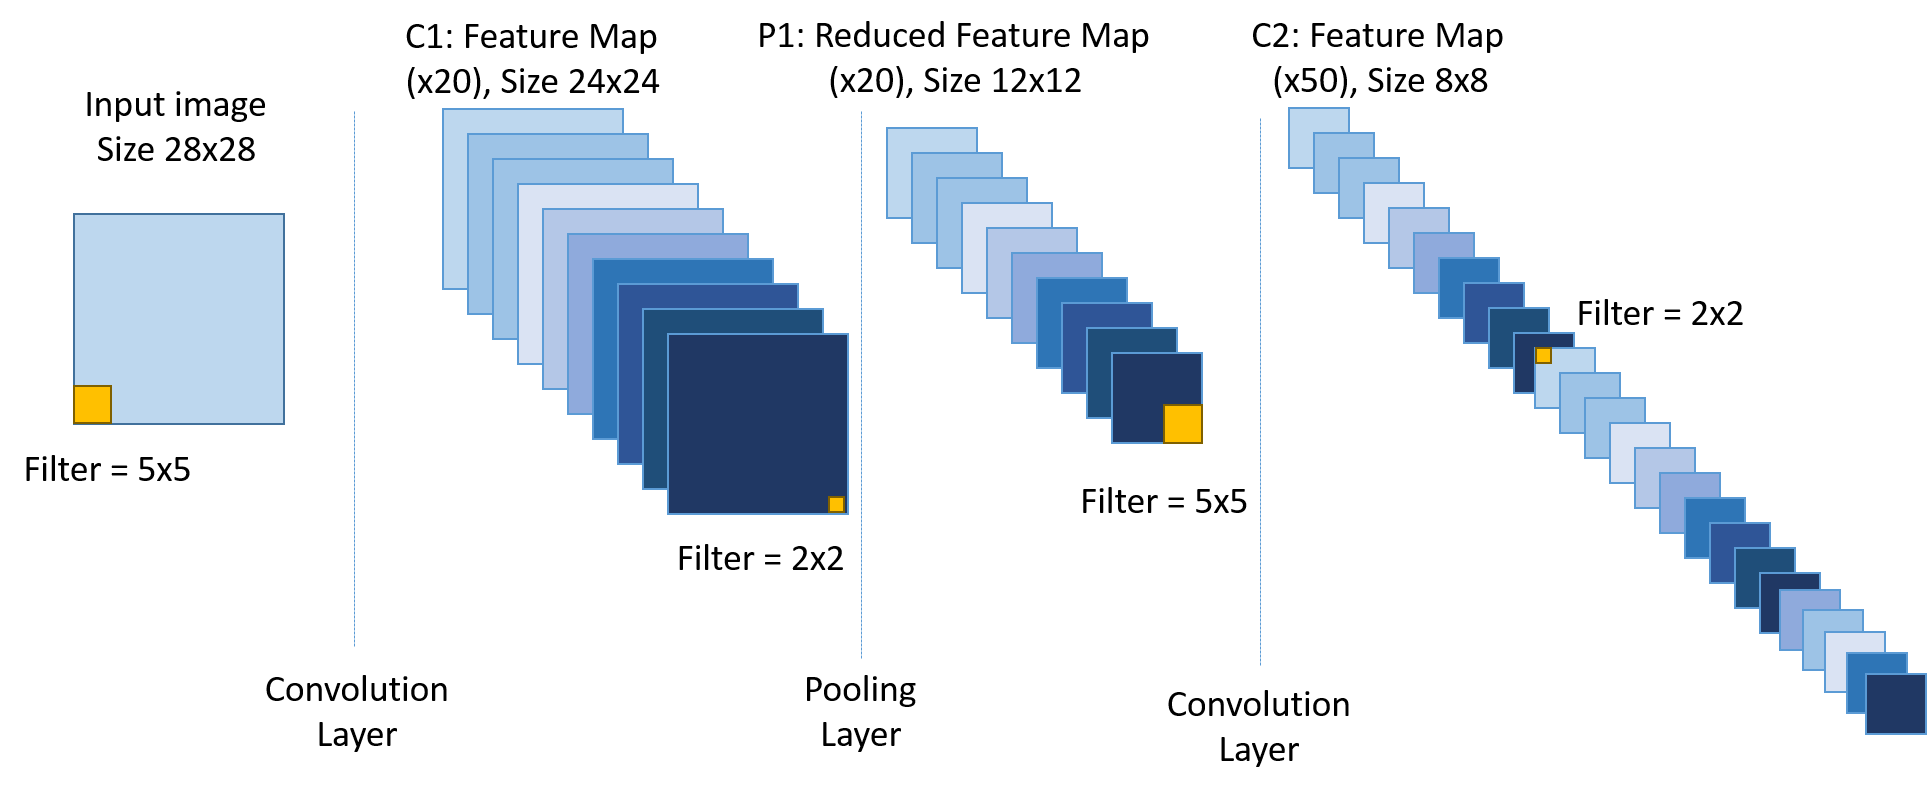
\includegraphics[width=13cm]{figures/Papaa_LeNet5-1.png}
\caption{Representation of the classification process - \textit{Part 1}}
\label{fig:cnn14}
\end{figure}

\begin{figure}[h!]
\centering
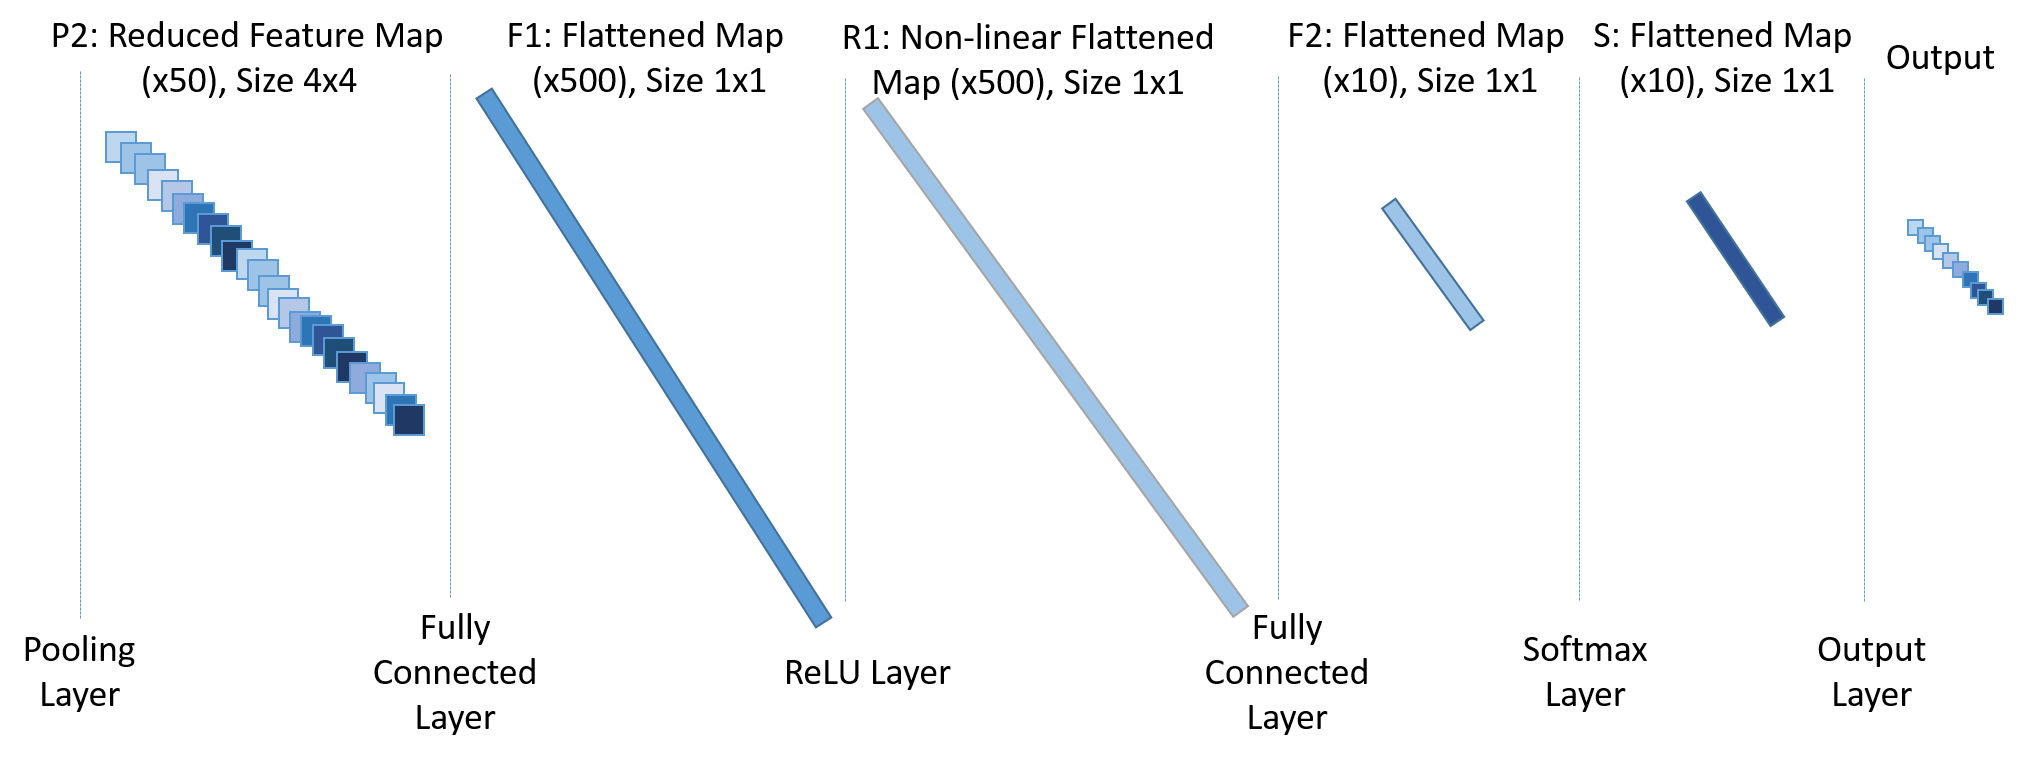
\includegraphics[width=\linewidth]{figures/Papaa_LeNet5-2.png}
\caption{Representation of the classification process - \textit{Part 2}}
\label{fig:cnn16}
\end{figure}

The following table indicates the use of various layers from the LeNet-5 architecture in this application. Each layer has an input size, output size and number of computations associated with it.\newline

\begin{table}[h!]
\centering
 \caption{Characterisitics of LeNet-5 layers in application using CNN to recognise hand-written digits}
 \vspace{3mm}
 \renewcommand\arraystretch{1.4}
 \begin{tabular}{ | m{7em} | c | c | c | c | r | }
 \hline
 \multicolumn{6}{|c|}{LeNet-5 CNN Application: Characterisitics layers} \\
 \hline
 \multicolumn{1}{|c|}{\bfseries Layer} & \multicolumn{1}{c|}{\bfseries Inputs} & \multicolumn{1}{c|}{\bfseries Outputs} & \multicolumn{1}{c|}{\bfseries Input Size} & \multicolumn{1}{c|}{\bfseries Output Size} & \multicolumn{1}{c|}{\bfseries Computations} \\
 \hline
 Convolution 1 & 1 & 20 & 28x28 & 24x24 & 1324800 \\
 \hline
 Pooling 1 & 20 & 20 & 24x24 & 12x12 & 80640 \\
 \hline
 Convolution 2 & 20 & 50 & 12x12 & 8x8 & 6812800 \\ 
 \hline
 Pooling 2 & 50 & 50 & 8x8 & 4x4 & 22400 \\
 \hline
 Inner Product 1 & 800 & 500 & 1x1 & 1x1 & 1600500 \\
 \hline
 ReLu & 500 & 500 & 1x1 & 1x1 & 500 \\
 \hline
 Inner Product 2 & 500 & 10 & 1x1 & 1x1 & 20010 \\
 \hline
 Softmax & 10 & 10 &  1 & 1 & 22 \\
 \hline
 \end{tabular}
 \label{table:mnist_layers_comp}
\end{table}
From Table \ref{table:mnist_layers_comp}, it can be calculated that the total number of computations performed by all the layers is \verb|9,861,672|. This is the number of computations required for a single image to be classified and recognised as a digit.

\subsection{Results}
\label{sect5_3_2}
The MNIST handwritten digit recognition application was executed on different devices - two CPUs and one GPU, and average timings were calculated for different parts in the execution of kernels. There is a total of eight kernels executing on the device, launched by the host one after the other. Each kernel corresponds to a layer, as show in Figures \ref{fig:cnn13} and \ref{fig:cnn14}. The convolutional and pooling kernels are launched with a 3D global size corresponding to the number of outputs and their sizes, while the ReLu, fully connected and Softmax layers are launched with a 1D global size corresponding to the number of outputs of the layer (mentioned in Table \ref{table:mnist_layers_comp}.  Also, the sequential variant of the code written in C++ was executed on the two CPUs, and timings were noted. \newline\newline
The following results were obtained on Intel(R) Core(TM) i3-2350M, Intel(R) Xeon(R) E5-1650 CPU, and NVIDIA Quadro 600 GPU.

\begin{table}[h!]
\centering
 \caption{Execution time (in µs) for different operations in MNIST Application on different devices}
 \vspace{3mm}
 \renewcommand\arraystretch{1.6}
 \begin{tabular}{ | m{12em} | r | r | r |  }
 \hline
 \multicolumn{4}{|c|}{LeNet-5 CNN Application: OpenCL Execution Times} \\
 \hline
 \multicolumn{1}{|c|}{\bfseries Device} & \multicolumn{1}{c|}{\bfseries i3-2350M} & \multicolumn{1}{c|}{\bfseries E5-1650} & \multicolumn{1}{c|}{\bfseries Quadro 600} \\
 \hline
 Initialize Application & 1.6 & 1.3 & 1.5 \\
 \hline
 Allocate Host Memory & 17.2 & 16.9 & 16.5 \\
 \hline
 Initialize Device & 81058.2 & 78408.9 & 36985.2 \\ 
 \hline
 Build Kernel & 152719.7  & 130634.2 & 16914.6 \\
 \hline
 Allocate Device Memory & 1312.1  & 1025.2 & 1364.7 \\
 \hline
 OpenCL Kernel Execution &1223.8 &  397.7 & 3903.5 \\
 \hline
 Sequential Execution & 85523 &  33892 & \textit{Not Applicable} \\
 \hline
 \end{tabular}
 \label{table:mnist_timings}
\end{table}
%Kernel Execution &12223.8 & 16251.4 & 18930.7 & 15581.6 & 3903.5 \\

\subsection{Performance Analysis}
\label{sect5_3_3}
The results above in Table \ref{table:mnist_timings} show the time taken on three different processors for initializing the application, allocating memory in the host, initializing the device on which the kernels will execute, building the kernels, allocating memory on the device, and the execution of all kernels. The sequential execution timing indicates the time taken by the CPU to run the C++ code for digit recognition.

\subsubsection*{Performance in GOPS}
\label{sect5_3_3_a}
Based on the total number of computations found out in Section \ref{sect5_3_1} and execution times in Table \ref{table:mnist_timings}, the performance of the devices was calculated in Giga Operations Per Second (\ac{GOPS}). The following formula was used to derive this value:
\[Performance \, in \, GOPS=\frac{Number \, of \, computations}{Execution \, time \, in \, ns}\]

\begin{table}[h!]
\centering
 \caption{Execution time (in µs) for different operations in MNIST Application on different devices}
 \vspace{3mm}
 \renewcommand\arraystretch{1.6}
 \begin{tabular}{ | m{12em} | r | r | r |  }
 \hline
 \multicolumn{4}{|c|}{LeNet-5 CNN Application: Performance in GOPS} \\
 \hline
 \multicolumn{1}{|c|}{\bfseries Device} & \multicolumn{1}{c|}{\bfseries i3-2350M} & \multicolumn{1}{c|}{\bfseries E5-1650} & \multicolumn{1}{c|}{\bfseries Quadro 600} \\
 \hline
 Sequential Execution & 0.115 &  0.291 & \textit{Not Applicable} \\\hline
 OpenCL Kernel Execution & 8.06 &  24.79 & 2.53 \\
 
 \hline
 \end{tabular}
 \label{table:mnist_gops}
\end{table}

\subsubsection*{Discussion}
\label{sect5_3_3_b}

Comparing the timing values for the CPUs from Tables and \ref{table:mnist_timings}, the extent of parallelism introduced by OpenCL can be evidently noticed. There is a speedup of 69 times for Intel(R) Core(TM) i3-2350M and 85 times for Intel(R) Xeon(R) E5-1650. \newline\newline
As evident from Table \ref{table:mnist_gops}, the performance of Intel(R) Xeon(R) E5-1650 CPU running OpenCL kernels is the best at 24.79 GOPS, followed by Intel(R) Core(TM) i3-2350M at 8.06 GOPS and then by NVIDIA Quadro 600 GPU at 2.53 GOPS. This can be attributed to the device characteristics, which were queried using provided APIs by OpenCL seen as follows:

\begin{figure}[h!]
\centering
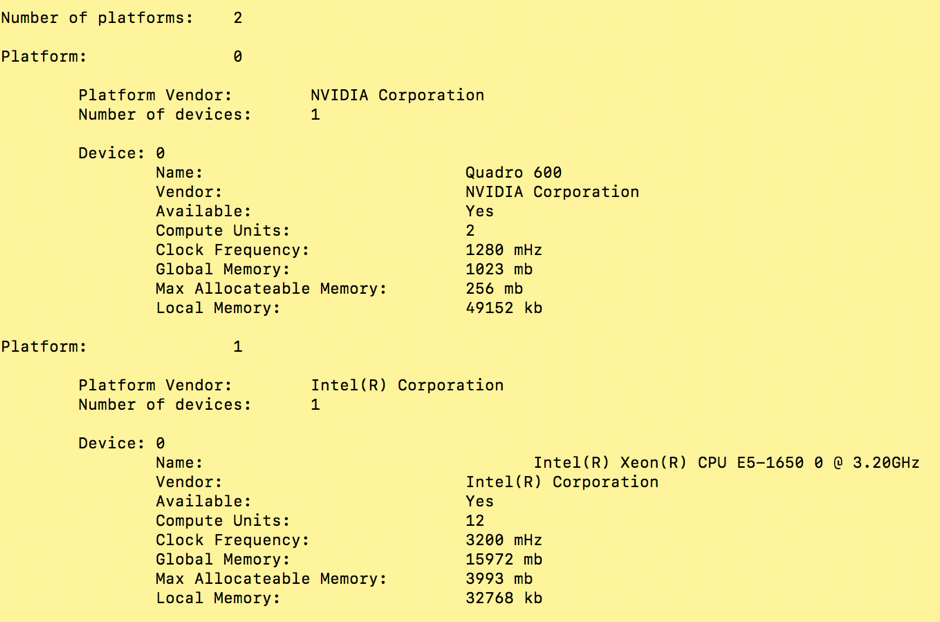
\includegraphics[width=11cm]{figures/Devquery.png}
\caption{Device characterisitcs of Intel Xeon E5-1650 CPU and NVIDIA Quadro 600 CPU}
\label{fig:cnn17}
\end{figure}

Due to higher number of compute units (12) for the CPU, OpenCL is able to parrallelise the code to a much greater extent, as compared to the GPU (2). Also, the clock frequency at which the CPU can execute at (3.2 GHz) is much higher than that of  the GPU (1.28 GHz). Thus, the CPU shows better performance in executing OpenCL parallelised code.